%!TeX root = RJwrapper.tex

\title{{psvmSDR}: An R Package for a Unified Algorithm for Sufficient Dimension Reduction via Principal Machines}
\author{by Jungmin Shin, Seung Jun Shin and Andreas Artemiou}

\maketitle

\abstract{
Sufficient dimension reduction (SDR), which seeks a lower-dimensional subspace of the predictors containing regression or classification information, has been popular in a machine learning community. In this work, we present a new R software package \CRANpkg{psvmSDR} that implements a new class of SDR estimators, which we call the principal machine (PM) generalized from the principal support vector machine (PSVM). The package covers both linear and nonlinear SDR and provides a function applicable to realtime update scenarios. The package implements the descent algorithm for the PMs to efficiently compute the SDR estimators in various situations. This easy-to-use package will be an attractive alternative to the \CRANpkg{dr} R package that implements classical SDR methods.
}

\section{Introduction} \label{sec:INTRO}

Dimension reduction is essential in modern applications in statistics and machine learning as the data size grows. 
In this regard, the \strong{sufficient dimension reduction} \citep[SDR,][]{Li1991::sir,Cook1998::regr} has gained great popularity in supervised learning problems.
For a given pair of univariate response $Y$ and $p$-dimensional predictor $\bX$, SDR assumes 
\begin{equation} \label{eqn:linear_model}
Y \perp \mathbf{X} \mid \mathbf{B}^{\top} \mathbf{X},     
\end{equation}
where $\perp$ denotes statistical independence. Under \eqref{eqn:linear_model}, SDR seeks the minimal space spanned by $\bB \in \mathbb{R}^{p \times d}$, called the \dfn{central subspace}, and denoted by $\cs$ that contains complete regression information of $Y$ on $\bX$. We assume $\cs = \mbox{span}\{\bB\}$ in \eqref{eqn:linear_model}. The dimension of $\cs$, $d$ is also an important quantity to be estimated from the data. 

There are numerous SDR estimators to estimate $\cs$. Earliest proposals are based on an inverse moment, such as sliced inverse regression \citep[SIR,][]{Li1991::sir} and sliced average variance estimates \citep[SAVE,][]{Cook1991::save}. {Other methods are based on forward regression models, including principal Hessian directions \citep[pHd,][]{Li1992::phd} and minimum average variance estimation \citep[MAVE,][]{xia2002adaptive}.}
Several R packages are available for the practical implementation of these classical SDR methods. The \CRANpkg{dr} package \citep{weisberg2015dr}, for instance, concisely implements many of these techniques (e.g., SIR, SAVE, pHd). {Other packages such as \CRANpkg{itdr} \citep{itdr_package} and \CRANpkg{orthoDr} \citep{orthoDr_paper} also provide functions for various SDR approaches.}

The assumption \eqref{eqn:linear_model} is often called a linear SDR. \citet{Cook2007::nonlinear} generalized \eqref{eqn:linear_model}, and proposed a nonlinear SDR that pursues a function $\phi: \mathbb{R}^p \rightarrow \mathbb{R}^d$ satisfying
\begin{equation}
\label{eqn:nonlinear_model}
Y \perp \mathbf{X} \mid \phi(\mathbf{X}).
\end{equation}
Nonlinear SDR methods have been developed by directly extending the classical inverse methods to Reproducing Kernel Hilbert Space \citep[RKHS,][]{aronszajn1950theory}. However, there is no hands-on R  package that implements them.

Meanwhile, \citet{Li2011::psvm} proposed the principal support vector machine (PSVM), a unified framework for both linear and nonlinear SDR, by connecting the SDR problem to the support vector machine \citep[SVM,][]{vapnik1999nature}. More importantly, PSVM can be easily generalized to other supervised machine learning approaches other than the SVM with the hinge loss. We call the class of SDR methods that generalizes the PSVM the \strong{principal machine} \citep[PM,][]{shin2024concise}. {The PM methods, such as PSVM as well as principal quantile regression \citep[PQR,][]{wang2018principal}, principal least squares SVM \citep[PLSSVM,][]{artemiou2021real}, and principal asymmetric $L_2$ regression \citep[PALS,][]{soale2022sufficient}, have reportedly outperformed classical SDR approaches.}

In this article, we develop an R package \CRANpkg{psvmSDR} that renders a simple gradient descent algorithm to compute a wide variety of the PMs in a unified framework. 
The package offers two main functions \code{psdr()} and \code{npsdr()} that compute a wide variety of PMs for linear and nonlinear SDR, respectively. In addition, it also has a function \code{rtpsdr()} that executes the realtime SDR estimation for streamed data. 

We highlight the main advantages of the package \CRANpkg{psvmSDR} in the following.
\begin{itemize}
\item It can solve both linear and nonlinear SDR problems in a unified framework using a simple and efficient gradient descent algorithm. 
\item It can be applied to a binary classification, where most inverse-moment-based approaches suffer.
\item It can compute a PM estimator with a user-specified arbitrary convex loss, adding flexibility to the methods. 
\item  It can handle streamed data by directly updating the SDR estimator without storing the entire data.  
\end{itemize}
The package is now available from CRAN at \url{https://cran.r-project.org/web/packages/psvmSDR} and can be installed from R with the following command:
\begin{example}
 > install.packages("psvmSDR")
\end{example}

The rest of the article is organized as follows. In Section \ref{sec:PSDR}, we introduce the principal machine (PM) under a linear,  nonlinear, and realtime SDR framework along with the corresponding functions \code{psdr()}, \code{npsdr()}, and \code{rtpsdr()}. In Section \ref{sec:optim}, we describe computational details about the package, and its efficiencies are investigated. In Section \ref{sec:overview}, we overview the package structure and explain how to implement the functions with examples. We conclude with a summary and discussion in Section \ref{sec:CON}.

\section{Principal machines: generalization of PSVM} \label{sec:PSDR}

We start by introducing the PSVM \citep{Li2011::psvm}. For a given sequence of $c_1 < c_2 < \cdots < c_h$, the PSVM minimizes the following objective function in the population level: 
\begin{equation} \label{eqn:model}
    (\alpha_{k}, \bbeta_{k}) = \argmin_{\alpha, \bbeta} \bbeta^{\top} \bSigma \bbeta + \lambda \E \left[\tilde{Y}_k \{\alpha + \bbeta^{\top} (\bX - \bmu)\}\right]_+, \quad k = 1, 2, \cdots, h,
\end{equation}
where $\bmu = \E(\bX)$, $\bSigma = \COV(\bX)$, and $[u]_+ = \max\{0, u\}$. Here $\tilde{Y}_{k}$ is a pseudo-binary response, taking 1 if $Y < c_k$ and $-1$ otherwise, and a positive constant $\lambda$ is a cost parameter whose choice is not overly sensitive for estimating $\cs$. \citet{Li2011::psvm} showed the unbiasedness of $\bbeta_{k}$, i.e., $\bbeta_{k} \in \cs, \forall k = 1, 2, \cdots, h$.  

It is important to note that convexity of the objective function in \eqref{eqn:model} is the only requirement for the PSVM to be unbiased, and this naturally leads to a generalized version of the PSVM, which we call the PM. We can categorize the PM into two types: one is response-based PM (RPM), and the other is loss-based PM (LPM). The RPM obtains multiple solutions by perturbing the pseudo-response $\tilde Y_k$, while the loss function remains unchanged. The PSVM belongs to this category. On the other hand, the LPM calculates multiple solutions by changing the loss functions, while the pseudo-response $Y_k$ is fixed as $Y$ for all $k$. The principal weighted support vector machine \citep[PWSVM,][]{shin2017principal} and the principal quantile regression \citep[PQR,][]{wang2018principal} are the earliest proposals of the LPM.  

\subsection{2.1 Linear principal machines} \label{sec:LPSDR}

The linear PM solves
\begin{align} \label{eqn:pm}
(\alpha_{k}, \bbeta_k) = \argmin_{\alpha, \bbeta} \bbeta^\top \bSigma\bbeta + \lambda \E \left[L_{k} \left\{\tilde Y_k, f(\bX)\right\} \right], \qquad k = 1, 2, \cdots h,
\end{align}
where $f(\bX) = \alpha + \bbeta^\top (\bX - \bmu)$ and $L_k(y, f)$ denotes a convex loss function of a margin, $yf$ for a binary $y \in \{-1, 1\}$ or residual $y - f$ for a continuous $y \in \mathbb{R}$. The RPM solves \eqref{eqn:pm} for different values of $\tilde Y_k$ over $k$ to obtain multiple solutions while keeping $L_k$ fixed as, say, $L$. On the other hand, the LPM  solves it with different loss functions $L_k$ while a pseudo-response $\tilde Y_k$ remains fixed as the original response $Y$. For instance, PWSVM, the first proposal under the LPM framework, solves \eqref{eqn:pm} using the loss function $L_k(y, f) = \pi_k(y)[1 - yf]_+$, where $\pi_k(y) = c_k$ if $y = 1$, and $\pi_k(y) = 1 - c_k$ otherwise, for a given $c_k \in (0,1)$ while $\tilde Y$ is fixed as $Y \in \{-1, 1\}$. The PWSVM is proposed for SDR in binary classification problems, addressing the limitations of PSVM when the dimensionality $d > 1$.

Given $(y_i, \bx_i), i = 1, 2, \cdots, n$, the sample counter part of \eqref{eqn:pm} is
\begin{equation}
\label{eqn:sample_model}
(\hat \alpha_k, \hat \bbeta_k) = \argmin_{\alpha, \bbeta} \bbeta^{\top} \hat \bSigma \bbeta + \frac{\lambda}{n} \sumi  L_k\left(\tilde y_{k,i}, \alpha + \bbeta^\top \bz_i \right), \qquad k = 1, 2, \cdots h,
\end{equation}
where $\bz_i = \bx_i - \sumi \bx_i/n$ and $\hat \bSigma = n^{-1}\sumi \bz_i \bz_i^\top$ denotes a sample covariance matrix. The PM working matrix is then 
\begin{equation} \label{eqn:working_matrix}
\hat{\mathbf{M}} = \sum_{k=1}^h \hat{\boldsymbol{\beta}}_{k} \hat{\boldsymbol{\beta}}_{k}^{\top},
\end{equation}
and its first $d$ eigenvectors of $\hat \bM$ estimate $\bB$ under \eqref{eqn:linear_model}, where $d$ denotes the dimension of $\cs$, often called the \dfn{structural dimension}.
The \CRANpkg{psvmSDR} package offers \code{psdr()} function to compute the linear PM estimates with a given loss function. 

In the linear SDR, it is also crucial to estimate the structural dimension  $d$. The linear PM employs the following BIC-type criterion proposed by \citet{Li2011::psvm} to estimate $d$:
\begin{equation}\label{eqn:structure dimension}
\hat{d}=\underset{d \in\{1, \cdots, p\}}{\operatorname{argmax}} \sum_{j=1}^{d} v_{j}-\rho \frac{d \log n}{\sqrt{n}} v_{1},
\end{equation}
where $v_{1} \geq \cdots \geq v_{p} (p > d)$ are eigenvalues of $\hat{\mathbf{M}}$ in \eqref{eqn:working_matrix}, with $\rho$ being a hyperparameter that can be chosen in a data-adaptive manner. The \CRANpkg{psvmSDR} package contains \code{psdr\_bic()} function for estimating $d$ based on \eqref{eqn:structure dimension}.

There are numerous PMs by employing a variety of convex loss functions in supervised learning problems. 
For RPMs, the principal logistic regression with negative log-likelihood loss \citep[PLR,][]{shin2017penalized}, the principal $L_q$-SVM with $L_q$ hinge loss \citep[$L_q$-PSVM,][]{artemiou2016sufficient}, and the principal least square SVM with the squared loss \citep[PLSSVM,][]{artemiou2021real} are proposed.
For LPMs, \citet{wang2018principal} suggested the principal quantile regression (PQR) with the check loss, \citet{kim2019principal} proposed the principal weighted logistic regression (PWLR), \citet{soale2022sufficient} introduced the principal asymmetric least square regression (PALSR) with the asymmetric least square loss, and \citet{jang2023principal} proposed the principal weighted least square SVM (PWLSSVM).

Table \ref{tbl:loss} provides a complete list of PMs implemented in \CRANpkg{psvmSDR} with the corresponding loss functions. 

\begin{table}[!tb]\onehalfspacing
    \centering
    \resizebox{\textwidth}{!}{
    \begin{tabular}{clcllc} \hline
                    Type & Method   & Response & Margin (Residual)   & Loss & \code{loss} \\ \hline
         \multirow{4}*{ RPM } &   SVM & \multirow{4}*{
         $\begin{array}{cc}
         Y \in \mathbb{R},\\
         \tilde{Y}_k = \mathds{1}\{Y \ge c_k\} \\
         \qquad~~ - \mathds{1}\{Y < c_k\}
         \end{array}$}     &   \multirow{4}*{$m_k = \tilde Y_k f$}  & ${[1-m_k]}_+$ & \code{`svm'} \\ 
                         & Logistic  &      &               & $\log(1 + e^{-m_k})^{-1}$ & \code{`logit'}\\ 
                        & $L_2$-SVM    &    &                & $\{[1-m_k]_+\}^2$ & \code{`l2svm'}\\ 
                         & LS-SVM &      &                & $[1-m_k]^{2}$ & \code{`lssvm'}\\ \hline 
         \multirow{6}*{LPM}& WSVM    & \multirow{4}*{${Y = \tilde Y_k \in \{-1,1\}}$}    &  \multirow{4}*{$m = Yf$}        & $\pi_{k}(Y)[1-m]_+$ & \code{`wsvm'}\\ 
                         & Wlogistic  &      &               & $\pi_{k}(Y)\log(1 + e^{-m})^{-1}$ & \code{`wlogit'}\\ 
                        & W$L_2$-SVM    &    &               & $\pi_{k}(Y)\{[1-m]_+\}^2$ & \code{`wl2svm'} \\ 
                         & WLS-SVM &      &                & $\pi_{k}(Y)[1-m]^{2}$ & \code{`wlssvm'}\\ \cline{2-6} 
                         & Quantile  & \multirow{2}*{${Y = \tilde Y_k \in \mathbb{R}}$}    &\multirow{2}*{$r = Y - f$}  & $r \{c_k - I(r<0)\}$& \code{`qr'}\\
                         &Asym. LS  &  &    & $r^2 \{c_k - I(r<0)\}$ & \code{`asls'}\\ \hline
    \end{tabular}} \\
    \caption{Different types of the convex loss functions available in the package \CRANpkg{psvmSDR}. The column \code{loss} indicates a specific syntax of the argument that is passed to \code{psdr()} and \code{npsdr()} to implement the corresponding methods.}
    \label{tbl:loss}
\end{table}

\subsection{2.2 Kernel principal machines for nonlinear SDR} \label{sec:NLPSDR}

A nonlinear generalization of \eqref{eqn:pm} under \eqref{eqn:nonlinear_model} is
\begin{equation}\label{model:non_pm_population}
(\alpha_{0,k}, g_{0,k}) = \argmin_{\alpha \in \mathbb{R}, g \in \mathcal{H}} \VAR \{\psi(\bX)\}+\lambda \E\left[ {L}_k \left\{ \tilde{Y}_{k}, f(\bX) \right\} \right], \qquad k = 1, 2, \cdots, h,
\end{equation}
where $f(\bX)=\alpha+g(\bX)-\E\{g(\bX)\}$ with $g$ being a function in a Hilbert space $\mathcal{H}$ of functions of $\bX$. 
Let $(\alpha_{0,k}, g_{0,k})$ be the minimizer of \eqref{model:non_pm_population}, then $g_{0,k}(\bX)$ is necessarily a function of the sufficient predictor $\phi(\bX)$ in \eqref{eqn:nonlinear_model} and its unbiasedness for the nonlinear SDR is established by \citet{Li2011::psvm}.

Employing the reproducing kernel Hilbert space (RKHS) generated by a positive definite kernel $K(\cdot, \cdot)$ for the space of $g$, we have the following finite-dimensional basis representation of $g$:
\begin{align}\label{eqn:fx}
g(\bx) = \sum_{j=1}^b \beta_j \left\{\psi_{j}(\mathbf{x})- \bar \psi_j \right\}
\end{align}
with 
\begin{align}\label{eqn:psi_gen}
\psi_j(\mathbf{x})=\left\{\mathbf{k}(\mathbf{x})\right\}^{\top} \mathbf{q}_j / \lambda_j, \quad j=1, \cdots b, \qquad \mbox{and} \qquad \bar \psi_j = \sum_{i=1}^{n}\psi_{j}\left(\mathbf{x}_{i}\right)/n,
\end{align}
where $\mathbf{k}(\cdot)=\{K(\cdot, \bx_i) : i=1,\ldots,n\}^{\top}$, and $\mathbf{q}_j$ and $\lambda_j$ are the $j$th leading eigenvector and eigenvalue of the centered kernel matrix $\mathbf{K} = \{K_{ij}\} \in \mathbb{R}^{n\times n}$ with $K_{ij} = K(\bx_i, \bx_j) - \sum_{k = 1}^n K(\bx_k, \bx_j)/n$. We refer Section 6 of \citet{Li2011::psvm} for the theoretical justification for \eqref{eqn:fx} and \eqref{eqn:psi_gen}.  In \CRANpkg{psvmSDR}, we employ the radial/Gaussian kernel and set $b = n/3$ as recommended by \citet{Li2011::psvm}. 

By employing \eqref{eqn:fx}, the sample counter part of \eqref{model:non_pm_population} is 
\begin{equation}\label{eqn:sample_nonlinear_pm}
(\hat \alpha_k, \hat \bbeta_k) = \argmin_{\alpha, \bbeta} {\bbeta}^{\top} \hat \bSigma {\bbeta}+\frac{\lambda}{n} 
   \sum_{i=1}^{n} L_{k} \left( \tilde{y}_{k,i}, \alpha + {\bbeta}^{\top} \bz_{i} \right), \qquad k = 1, 2, \cdots, h,   
\end{equation}
where $\bz_i = \sum_{j=1}^b \psi_{j}(\mathbf{x}_i)- \bar \psi_j$ and $\hat \bSigma = n^{-1} \sumi \boldsymbol{\bz}_i \boldsymbol{\bz}_i^{\top}$. We note that this kernel PM in \eqref{eqn:sample_nonlinear_pm} is also linear in the parameter, exactly the same as the linear PM \eqref{eqn:sample_model}. 
For a given $\bx$, one can compute the sufficient predictors, $\hat{\phi}(\bx)=\hat{\bV}^{\top}\left\{ \psi_1(\bx), \ldots,  \psi_b(\bx)\right\}^{\top}$, where $\hat{\bV}$ denotes the $d$-leading eigenvectors of $\sum_{k=1}^h \hat{\bbeta}_{k} \hat{\bbeta}_{k}^{\top}$. The \CRANpkg{psvmSDR} package offers \code{npsdr()} function to compute the nonlinear PM estimates.

\subsection{2.3 Principal least square machines for realtime SDR} \label{sec:rtPSDR}
When data is collected in a streamed fashion, it is prohibitive to use all data to compute the SDR estimator due to memory constraints. Therefore, it is important to develop real-time SDR algorithms that directly update the SDR estimators without storing the entire data. In this regard, \citet{artemiou2021real} proposed PLSSVM which solves \eqref{eqn:pm} with the squared loss $L(\tilde y, f) = (1 - \tilde y f)^2$.

Let's consider the following scenario. In addition to the currently available (old) data $\mathbb{D}_{\texttt{O}} = (y_i, \bx_i), i = 1, 2, \cdots, n$, suppose $m$ additional (new) data $\mathbb{D}_{\texttt{N}} = (y_i, \bx_i), i = n+1, \cdots, n+m$ arrives. Let $\mathbb{D}_{\texttt{W}} = \mathbb{D}_{\texttt{O}} \cup \mathbb{D}_{\texttt{N}}$ denote the whole data. The subscripts $\texttt{O}, \texttt{N}$, and $\texttt{W}$ are used to denote the quantities related to old, new, and whole data, respectively.  
\citet{artemiou2021real} showed that the PLSSVM solution for the whole data, ${\br}_{\texttt{W}} = (\hat{\alpha}_{\texttt{W}},\hat {\bbeta}_{\texttt{W}}^\top)^\top\in \mathbb{R}^{p+1}$, is given by
\begin{align}\label{eqn:rtpsdr_coef}
\br_{\texttt{W}} = \{\bI - \bA_{\texttt{O}}^{-1} \bB_{\texttt{N}} (\bI + \bA_{\texttt{O}}^{-1} \bB_{\texttt{N}})^{-1} \} ( \br_{\texttt{O}} + \bA_{\texttt{O}}^{-1}\mathbf{c}_{\texttt{N}} ),
\end{align}
where $\br_{\texttt{O}}$ is the solution for $\mathbb{D}_{\texttt{O}}$, and $\bA_{\texttt{O}}^{-1} \in \mathbb{R}^{{(p+1)}\times {(p+1)}}$ is also computable from $\mathbb{D}_{\texttt{O}}$, while $\bB_{\texttt{N}} \in \mathbb{R}^{{(p+1)}\times {(p+1)}}$ and $\mathbf{c}_{\texttt{N}} \in \mathbb{R}^{p+1}$ are computable from $\mathbb{D}_{\texttt{N}}$. That is, one can directly update $\br_{\texttt{W}}$ from $\br_{\texttt{O}}$ without storing the entire $\mathbb{D}_{\texttt{O}}$, but $\bA_{\texttt{O}}$ only. We remark that $\bA_{\texttt{W}}$ can be directly updated from $\bA_{\texttt{O}}$ and the new data, and its computational complexity does not depend on the size of $\mathbb{D}_\texttt{O}$. We refer Section 3 of \citet{artemiou2021real} for the exact forms of these quantities.

The \CRANpkg{psvmSDR} package offers \code{rtpsdr()} that implements the realtime SDR using PLSSVM for a continuous response as well as PWLSSVM by \citet{jang2023principal} for a binary response.

\section{Computation}\label{sec:optim}
In this section, we describe computational details about \code{psdr()} and \code{npsdr()} in \CRANpkg{psvmSDR}.
Slightly abusing notation as $\bbeta^\top = \left(\alpha, \bbeta^\top\right)$ and $\bz_i^\top = \left(1, \bz_{i}^\top \right)$, the objective functions \eqref{eqn:sample_model} and \eqref{eqn:sample_nonlinear_pm} are then rewritten as
\begin{align} \label{eqn:obj}
L(\bbeta) = \bbeta^\top \mbox{Diag}\left\{0, \hat \bSigma\right\} \bbeta + \frac{\lambda}{n}\sumi L_k\left(\tilde y_{k,i}, \bbeta^\top \bz_i \right).
\end{align}
We propose the coordinatewise gradient descent (CGD) algorithm to minimize $L(\bbeta)$ in \eqref{eqn:obj}, which updates $\bbeta$ coordinatewisely as follows until converge:
\begin{align*}
\beta_j & \leftarrow \beta_j - \eta \frac{\partial L(\bbeta)}{\partial{\beta_j}}, ~~ j= 0, 1, 2, \cdots, p,
\end{align*}
where $\eta > 0$ denotes a learning rate determined by the user. 
We remark that some loss functions, such as the hinge loss and check loss are not theoretically differentiable at most finite number of points while numerically differentiable. 
{In practice, the CGD implementation ensures stable updates for non-smooth functions by employing analytical subgradients for built-in losses (e.g., hinge, quantile) and numerical approximations for user-defined losses.} 
The two main functions \code{psdr()} and \code{npsdr()} in \CRANpkg{psvmSDR} solve linear and nonlinear PMs via this CGD algorithm, respectively, and cover a wide variety of PM estimators by simply changing the loss functions (via \code{`loss'} argument) as listed in Table \ref{tbl:loss}. The CGD algorithm is easily extended to any user-defined convex loss function, since the corresponding derivative can be readily evaluated numerically. Both functions can take the name of the user-defined-loss function object as the \code{loss} argument which brings further flexibility to the PM estimators. 

\begin{figure}[!t]
     \centering
     \begin{subfigure}[b]{0.48\textwidth}
         \centering
        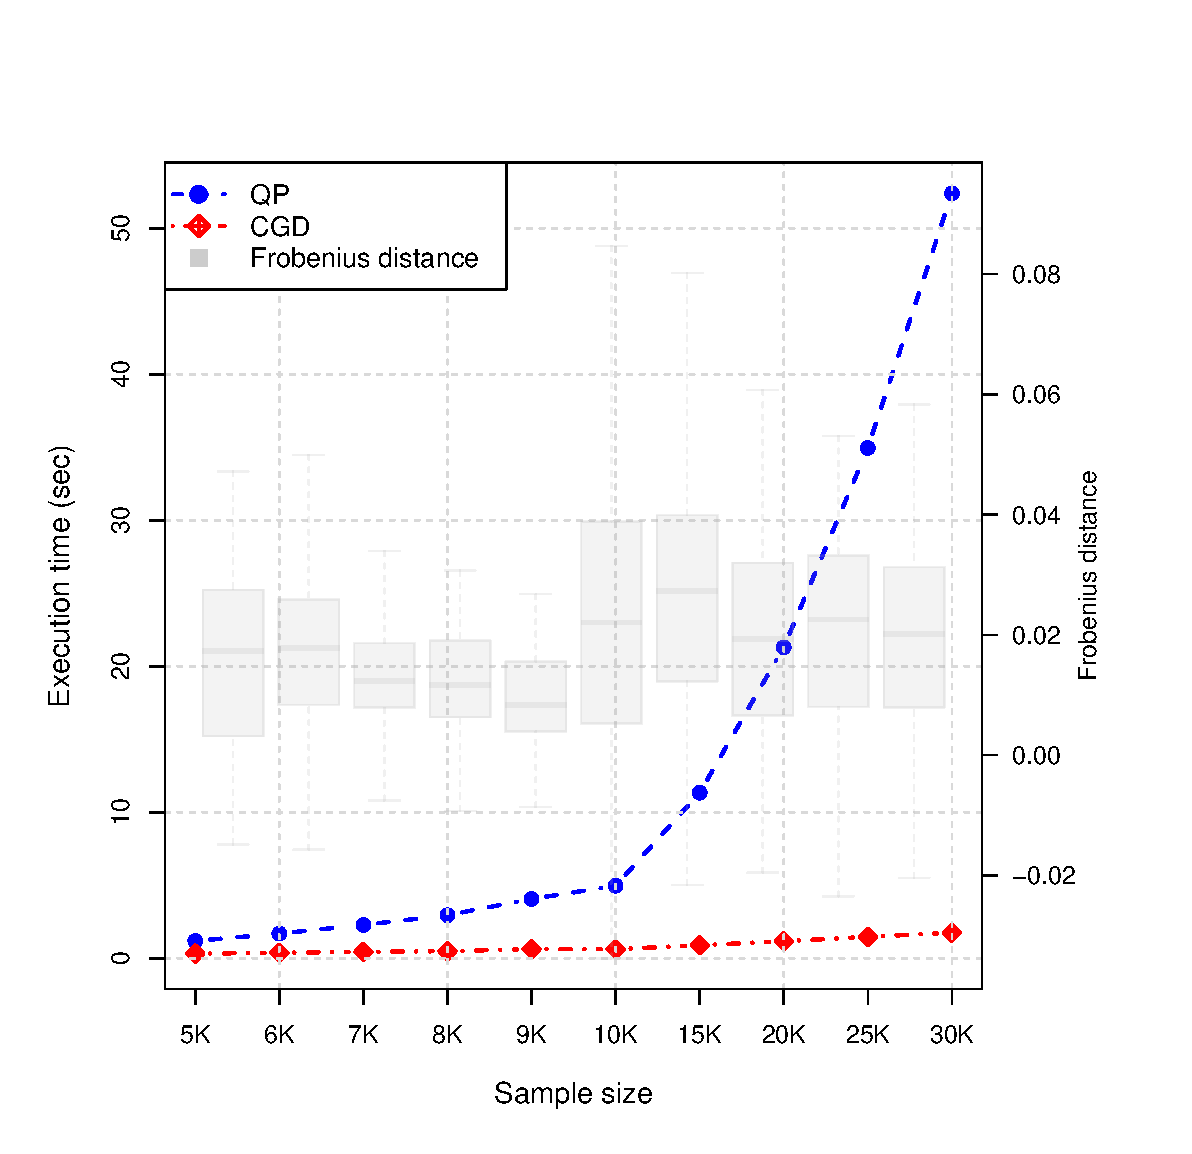
\includegraphics[width=1\textwidth]{comp_time_linear_revised_pdf.pdf}
        \caption{Linear PSVM}
        \label{fig:linear_time}
     \end{subfigure}
     \hfill
     \begin{subfigure}[b]{0.48\textwidth}
         \centering
        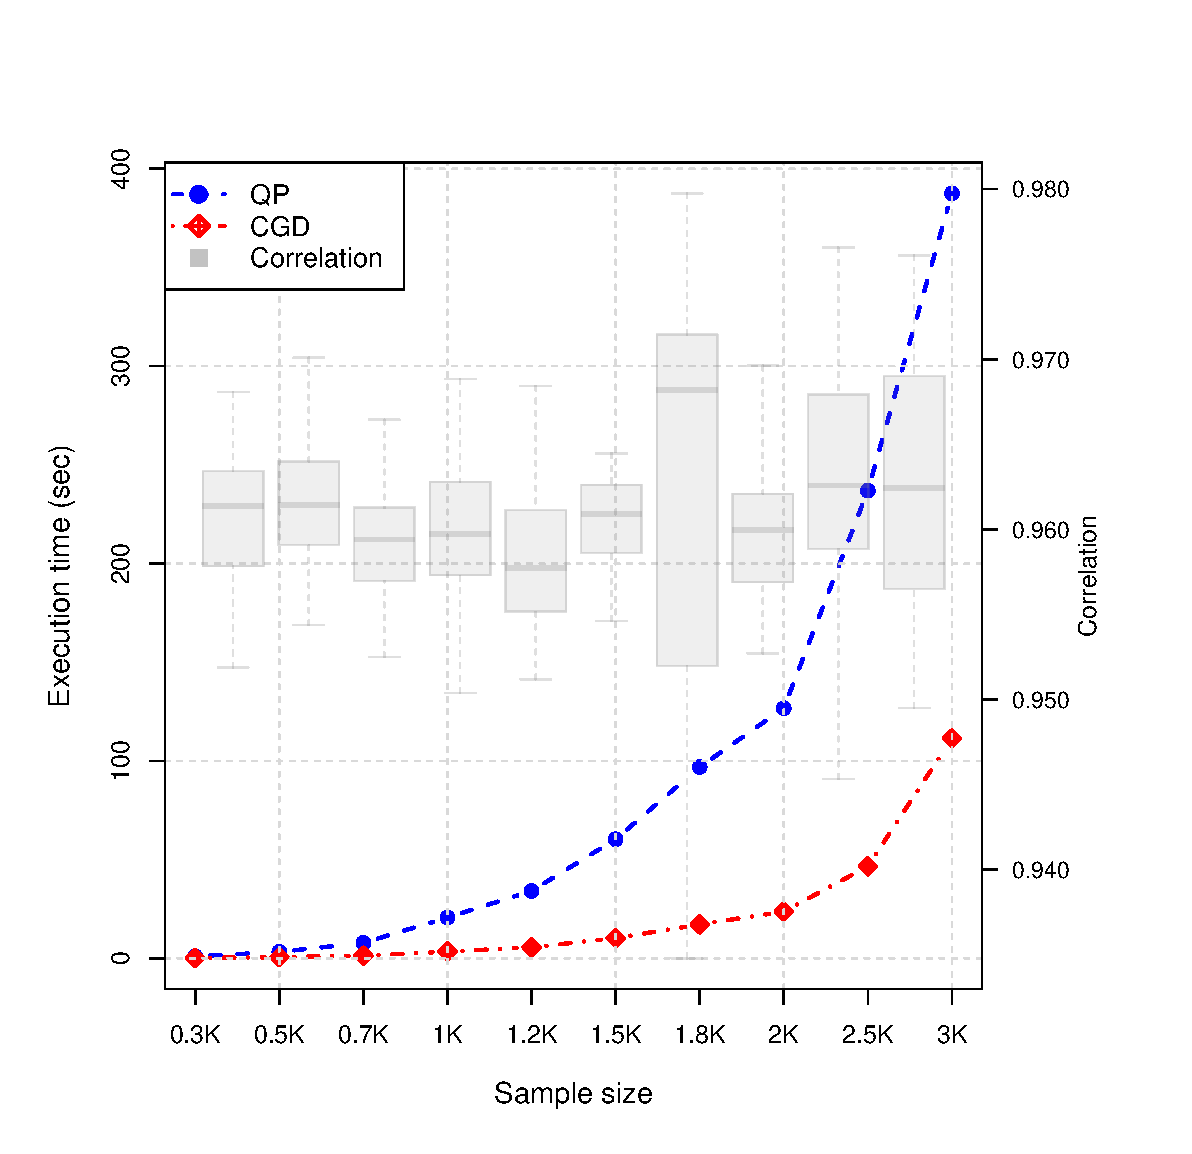
\includegraphics[width=1\textwidth]{comp_time_nonlinear_revised_pdf.pdf}
        \caption{Kernel PSVM}
        \label{fig:nonlinear_time}
     \end{subfigure}
	\caption{Average computing times of the QP and CGD algorithms over 100 repetitions are shown. The left and right panels correspond to the linear and kernel PSVM results, respectively. The blue and red dashed lines denote QP and CGD, respectively, illustrating the superior scalability of CGD. Overlaid gray boxplots depict estimation agreement measured by Frobenius distance for the linear case and prediction correlation for the nonlinear case.} 
	\label{fig:comparison_methods}
\end{figure}

{Each CGD iteration costs $\mathcal{O}(np)$ for the linear PM (\code{psdr()}) and $\mathcal{O}(nb)$ for the nonlinear PM (\code{npsdr()}), where $p$ is the data dimension and $b$ is the number of kernel basis functions used for the RKHS expansion in \eqref{eqn:psi_gen} \citep{luo1992convergence, tibshirani2007cd}. Following the empirical recommendation of \citet{Li2011::psvm}, we set $b$ between $n/3$ and $2n/3$ in practice.
In contrast, quadratic programming (QP) approaches for SVM-like objectives (e.g., \CRANpkg{kernlab}) have worst-case polynomial time $\mathcal{O}(n^{3}p^{3})$ (or $\mathcal{O}(n^{3}b^{3})$ for kernel PMs) \citep{platt1998sequential, cristianini2000introduction}, which scale less favorably as $n$ grows.}

To evaluate the computational efficiency of the proposed CGD algorithm, we compare its computing times for both linear and nonlinear (kernel) PSVM estimators to \code{ipop()} function in \CRANpkg{kernlab}, a standard QP solver for the SVM over 100 independent repetitions. A toy data is generated from the following regression model:
\begin{align}\label{model_regression_1}
y_i = x_{i1} / \left\{0.5+\left(x_{i2} + 1\right)^2\right\} + 0.2\epsilon_i,
\end{align}
where both $x_{ij}$ and $\epsilon_i$ are i.i.d. random samples from $N(0,1)$ for $i = 1, \cdots, n$ and $j = 1, 2, \cdots, 5$. Different sample sizes $n$ are considered from $5,000$ to $30,000$ for linear PSVM while from $300$ to $3,000$ for the kernel PSVM where the parameter dimension depends on $n$. 

{Figure~\ref{fig:comparison_methods} highlights the computational advantage of the CGD implementation, which achieves substantially lower runtimes than QP. In addition to runtime, we assessed estimation agreement. For the linear PSVM, we measured subspace similarity via the Frobenius distance between projection matrices, $|{\bP}_{\mathrm{CGD}} - {\bP}_{\mathrm{QP}}|_F$, where ${\bP} = \hat{\bB}(\hat{\bB}^{\top}\hat{\bB})^{-1}\hat{\bB}^{\top}$. For the kernel PSVM, predictive agreement is quantified by the correlation between fitted test responses, $ \mathrm{cor}(\hat{y}_{\mathrm{QP}}, \hat{y}_{\mathrm{CGD}})$, where $\hat{y}_{\mathrm{QP}}$ and $\hat{y}_{\mathrm{CGD}}$ are obtained from regressions of $y$ on the estimated sufficient predictors $\hat{\phi}_{\mathrm{QP}}(\bX)$ and $\hat{\phi}_{\mathrm{CGD}}(\bX)$. Across all sample sizes, the Frobenius distance remained near zero and the correlation close to one, confirming that CGD achieves accuracy indistinguishable from QP while being substantially faster.}

\section{Package overview and implementation}\label{sec:overview}
\subsection{4.1 Overview of the package \CRANpkg{psvmSDR}}
The \CRANpkg{psvmSDR} package is organized to allow users to run different types of PM methods in a unified fashion by calling just a few interface functions. Several auxiliary codes are then internally called to perform computations according to the options specified in those interface functions.
The overall design of \CRANpkg{psvmSDR} adopts the functional object-oriented programming approach \citep{chambers2014::R} with \code{S3} classes and methods. Every function in the package is either a wrapper that creates a single instance of an object or a method that can be applied to a class object.

The package can be installed and loaded in an R session via:
\begin{example}
 > install.packages("psvmSDR")
 > library("psvmSDR")
\end{example}
The main functions in the package are \code{psdr()} and \code{npsdr()}. 
These are designed to be analogous to linear and nonlinear principal sufficient dimension reduction methods, respectively. 
Each function returns an \code{S3} object, \code{`psdr'} and \code{`npsdr'}, respectively. 
Also, compatible \code{S3} methods \code{plot()} and \code{print()} let the users enjoy the result of dimension reduction through familiar generic functions. 
Moreover, some explicit methods of which are related to the main functions are also provided, such as \code{psdr\_bic()} and \code{npsdr\_x()}.

A function \code{rtpsdr()} implements the PLSSVM in a realtime fashion \citep{artemiou2021real,jang2023principal} discussed in Section~\ref{sec:rtPSDR}. Table \ref{tbl:ft_list} summarizes the main functions along with their compatible methods.
In the following subsections,  we demonstrate the general usage of the main functions and methods of \CRANpkg{psvmSDR} by the \code{S3} class of the function.

\begin{table}[!t]
\centering
\renewcommand{\arraystretch}{1.3}
\setlength{\tabcolsep}{6pt}
\begin{tabularx}{\textwidth}{m{1.8cm} X m{1.8cm} m{3.2cm}} 
\toprule
Function & Description & Class & Compatible methods \\
\midrule
\code{psdr()} & Basic function for applying linear PMs with various loss functions & \multirow{2}{*}{\code{`psdr'}} & \multirow{4}{*}{\shortstack[l]{\code{psdr\_bic()} \\ \code{plot.psdr()} \\ \code{print.psdr()} \\ \code{summary.psdr()}}} \\
\cmidrule(r){1-2}
\code{rtpsdr()} & Real-time sufficient dimension reduction through principal (weighted) least squares SVM & & \\
\midrule
\code{npsdr()} & Basic function for applying kernel PMs with various loss functions & \code{`npsdr'} & \shortstack[l]{\code{npsdr\_x()} \\ \code{plot.npsdr()} \\ \code{print.npsdr()} \\ \code{summary.npsdr()}} \\
\bottomrule
\end{tabularx}
\caption{Main functions and compatible methods in the \CRANpkg{psvmSDR} package.}
\label{tbl:ft_list}
\end{table}

\subsection{4.2 Functions for \code{S3} class `\code{psdr}'}\label{sec:class_psdr}

A function \code{psdr}() provides a unified interface for all linear PMs solved by the CGD algorithm.
The following arguments are used (some are mandatory) when calling \code{psdr}() function and they must be provided in the order that follows:
\begin{example}
> psdr <- function(x, y, loss = "svm", h = 10, lambda = 1, eps = 1e-5, max.iter = 100, 
                   eta = 0.1, mtype = "m", plot = FALSE) 
\end{example}

\begin{itemize}[itemsep=.1mm]
\item \code{x}: input matrix; each row is an observation vector. \code{x} should have 2 or more columns.
\item \code{y}: response vector, either can be continuous or $\{1, -1\}$-coded binary variable.
\item \code{loss}: name of loss function objects listed in Table \ref{tbl:loss}, or the name of a user-defined (convex) loss function object. 
\item \code{h}: unified control for slicing or weighting; either a positive integer (number of slices/weights) or a numeric vector of cutpoints in $(0,1)$.
\item \code{lambda}: cost parameter.
\item \code{eps}: stopping criterion of the CGD algorithm.
\item \code{max.iter}: maximum iteration number of the CGD algorithm.
\item \code{eta}: learning rate for the CGD algorithm.
\item \code{mtype}: a margin type, which is either margin (\code{"m"}) or residual (\code{"r"}) (See, Table~\ref{tbl:loss}). Only needed when a user-defined loss is used. The default is "m".
\item \code{plot}: boolean. If \code{TRUE}, scatter plots of $Y$ and sufficient predictors will be presented. 
\end{itemize}

The main function \code{psdr()} returns an object with \code{S3} class \code{'psdr'} including
\begin{itemize}
	\item \code{evalues}: eigenvalues of the estimated working matrix \eqref{eqn:working_matrix}.
	\item \code{evectors}: eigenvectors of the estimated working matrix \eqref{eqn:working_matrix}.
	\item \code{fit}: metadata (n, p, hyperparameters, per-slice iteration/convergence info, etc.).
\end{itemize}

To further illustrate how to use function \code{psdr()}, we reuse the toy example which is formulated in \eqref{model_regression_1} with $n=200$.

\begin{example}
 > set.seed(100) 
 > n <- 200; p <- 5 
 > x <- matrix(rnorm(n*p, 0, 1), n, p) 
 > y <- x[,1]/(0.5 + (x[,2] + 1)^2) + 0.2 * rnorm(n)   
\end{example}

We then can apply the PSVM \citep{Li2011::psvm} using function \code{psdr()} with calling the argument \code{loss = "svm"} (default value) as below: 
\begin{example}
 > obj <- psdr(x, y)
 > summary(obj)
 === Summary of psdr Object ===
 Loss function: svm 
 Sample size (n): 200  | Variables (p): 5  | Response type: continuous 
 Lambda: 1  | Eta: 0.1  | Eps: 1e-05  | Max.iter: 100 

 --- Eigen Decomposition of Working Matrix (M) ---
 Top eigenvalues (up to 10):
 [1] 0.7803 0.0451 0.0070 0.0013 0.0002

 Estimated Eigenvectors (columns = central subspace basis):
         [,1]    [,2]    [,3]    [,4]    [,5]
 [1,]  0.9963  0.0003 -0.0069  0.0792  0.0328
 [2,]  0.0020 -0.9578  0.1250 -0.1082  0.2352
 [3,] -0.0189 -0.2385  0.1258  0.5707 -0.7754
 [4,] -0.0451  0.1507  0.7675  0.4600  0.4178
 [5,]  0.0708  0.0553  0.6159 -0.6669 -0.4096

 --- Per-slice diagnostics ---
   slice iter converged          obj
 1     1   46      TRUE 6.468460e-06
 2     2   46      TRUE 6.112350e-06
 3     3   45      TRUE 5.661422e-06
 4     4   46      TRUE 4.309816e-06
 5     5   45      TRUE 4.690990e-06
 6     6   45      TRUE 5.603063e-06
 7     7   45      TRUE 6.321184e-06
 8     8   46      TRUE 5.886324e-06
 9     9   46      TRUE 6.368887e-06

 Convergence summary:
   Total iterations: 410  | All slices converged: TRUE 
\end{example}
The output eigenvectors correctly estimate the true basis vectors $\left(1, 0, 0, 0, 0\right)^{\top}$ and $\left(0, 1, 0, 0, 0\right)^{\top}$.
The \code{summary()} function returns a summary of a \code{psdr} object. More detailed usage of the function and its arguments is provided in the package manual.
The method \code{plot.psdr()} creates the scatter plots between response and the $j$-th sufficient predictors. 
\begin{example}
 > plot(obj, d=1, lowess=TRUE)
\end{example}
\begin{figure}[!t]
    \centering
    \includegraphics[width=.55\linewidth]{ex1_psdr.eps}
    \caption{Scatter plots of $Y$ versus the first sufficient predictor $\hat{B}_{1}^{\top} \mathbf{X}$ from the generic method \code{plot.psdr()}.}
    \label{fig:ex1_psdr}
\end{figure}
The argument \code{obj} is the object from the function \code{psdr()} which contains information on estimated $\cs$. The number of sufficient predictors to be plotted is specified by the argument \code{d} whose default value is 1. By default, a locally weighted scatterplot smoothing (LOWESS) curve is plotted, unless \code{lowess=FALSE} is specified. The argument \code{"$\ldots$"} allows for additional arguments to be passed to generic \code{plot()} function such as \code{main}, \code{cex}, \code{col}, \code{lty}, and etc.

Now, we generate binary response $\tilde y_i = \operatorname{sign}(y_i)$ from \eqref{model_regression_1} to illustrate the PWSVM \citep{shin2017principal}, an example of the LPM. One can apply PWSVM by letting \code{loss = "wsvm"}. 
\begin{example}
 > y.binary <- sign(y)
 > obj_wsvm <- psdr(x, y.binary, loss = "wsvm")
 > print(obj_wsvm)
 > plot(obj_wsvm)
\end{example}
\begin{example} 
 --- Principal Sufficient Dimension Reduction (linear) ---
 Loss: wsvm  | n: 200  p: 5  | Response: binary 
 Lambda: 1  | Eta: 0.1  | Max.iter: 100  | Converged: TRUE 

 Eigenvalues (first 5):  0.3864, 0, 0, 0, 0 

 Eigenvectors (columns are SDR directions):
         [,1]    [,2]    [,3]    [,4]    [,5]
 [1,]  0.9938 -0.0392  0.0572  0.0000  0.0869
 [2,]  0.0590  0.8544 -0.0892 -0.4531 -0.2308
 [3,] -0.0181 -0.4386 -0.2064 -0.8624  0.1449
 [4,]  0.0201  0.1295 -0.8786  0.2124  0.4071
 [5,]  0.0903 -0.2437 -0.4174  0.0762 -0.8674
 \end{example}

Figure~\ref{fig:ex1_wsvm} visualizes the classification performance with only two sufficient predictors estimated by PWSVM.
With only two sufficient predictors, the two classes are well separated.

\begin{figure}[!t]
     \centering
     \includegraphics[width=.55\linewidth]{ex1_wsvm.eps}  
    \caption{A scatter plot of the predicted projections on the first and second sufficient predictors, i.e., $\hat{b}_1^{T}\bX$, $\hat{b}_2^{T}\bX$, respectively, estimated by PWSVM with \code{loss=``wsvm''}. }
    \label{fig:ex1_wsvm}
\end{figure}

One of many advantages of \code{psdr()} is that it can adopt any convex user-defined loss function in addition to existing choices listed in Table \ref{tbl:loss}.
A basic syntax of the arbitrary loss function follows:
\begin{example}
 loss_name <- function(u, ...){ body of a function }
\end{example}
Argument \code{u} is a variable of a function  (any character is possible) and any additional parameters of the loss function can be specified via \code{...} argument.
For example, one can define "\code{mylogistic}" and apply it to the function \code{psdr()} by specifying \code{loss="mylogistic"}.
\begin{example}
 > mylogistic <- function(u) log(1+exp(-u))
 > obj_mylogistic <- psdr(x, y, loss="mylogistic")
 > print(obj_mylogistic)
\end{example}
\begin{example}
 --- Principal Sufficient Dimension Reduction (linear) ---
 Loss: mylogistic  | n: 200  p: 5  | Response: continuous 
 Lambda: 1  | Eta: 0.1  | Max.iter: 100  | Converged: TRUE 

 Eigenvalues (first 5):  0.0337, 0.0011, 3e-04, 1e-04, 0 

 Eigenvectors (columns are SDR directions):
         [,1]    [,2]    [,3]    [,4]    [,5]
 [1,]  0.9948 -0.0845  0.0499  0.0214 -0.0143
 [2,] -0.0910 -0.9651  0.1157  0.0039 -0.2165
 [3,] -0.0001 -0.2001  0.0673 -0.3248  0.9219
 [4,] -0.0444  0.1015  0.9337  0.3331  0.0712
 [5,] -0.0070 -0.1054 -0.3285  0.8849  0.3128
\end{example}

As aforementioned, \CRANpkg{psvmSDR} provides a function \code{psdr\_bic()} that implements the BIC-type criterion in \eqref{eqn:structure dimension}.
{Here, $\rho$ serves as a tuning parameter. To determine its optimal value, \code{psdr\_bic} employs a $K$-fold cross-validation procedure that selects the $\rho$ yielding the most stable dimension estimates across folds.} 

\noindent
Following arguments are mandatory when calling the \code{psdr\_bic()}:

\begin{example}
psdr_bic <- function(obj, rho_grid = seq(0.001, 0.05, length = 10), cv_folds = 5,
                      plot = TRUE, seed = 123, ...)
\end{example}

\begin{itemize}
\item \code{obj}: the output object from the main function \code{psdr()} 
\item \code{rho\_grid}: numeric vector of candidate $\rho$ values; the default is \code{seq(0.001, 0.05, length = 10)}.
\item \code{cv\_folds}: number of cross-validation folds used for stability evaluation (default = 5).
\item \code{plot}: Boolean. If \code{TRUE}, the plot of BIC values is depicted.  
\item \code{seed}: random seed for reproducibility.
\item \code{$\cdots$}: additional arguments to be passed to generic \code{plot()}.
\end{itemize}

The function \code{psdr\_bic()} returns an object with S3 class \code{'psdr\_bic'} containing
\begin{itemize}
	\item \code{rho\_star}: the selected tuning parameter $\rho$ that minimizes the cross-validated variation of dimension estimates.
	\item \code{d\_hat}: the estimated structural dimension corresponding to \code{rho\_star}.
	\item \code{G\_values}: a matrix of BIC-type criterion values evaluated over candidate $\rho$ values.
	\item \code{cv\_variation}: the variation (variance) of estimated dimensions across CV folds, used as a stability measure.
	\item \code{fold\_dhat}: the estimated dimensions obtained from each CV fold.
\end{itemize}

\noindent
The following code demonstrates the use of \code{psdr\_bic()}, which by default visualizes the BIC-type criterion curves as shown in Figure~\ref{fig:plot and Gn}.
\begin{example}
 > d.hat <- psdr_bic(obj, rho_grid=seq(0.05, 0.1, length=5), cv_folds=5)
 > print(d.hat)
 $rho_star
 [1] 0.05

 $d_hat
 [1] 2

 $G_values
           [,1]      [,2]      [,3]      [,4]      [,5]
 [1,] 0.1670058 0.1662087 0.1654117 0.1646147 0.1638176
 [2,] 0.1696176 0.1680236 0.1664295 0.1648354 0.1632414
 [3,] 0.1677601 0.1653690 0.1629779 0.1605868 0.1581957
 [4,] 0.1649097 0.1617216 0.1585334 0.1553453 0.1521572
 [5,] 0.1618201 0.1578349 0.1538497 0.1498645 0.1458794

 $cv_variation
 rho=0.0500 rho=0.0625 rho=0.0750 rho=0.0875 rho=0.1000 
        0.0        0.2        0.3        0.3        0.0 

 $fold_dhat
      rho=0.0500 rho=0.0625 rho=0.0750 rho=0.0875 rho=0.1000
 [1,]          2          2          2          2          1
 [2,]          2          2          2          2          1
 [3,]          2          1          1          1          1
 [4,]          2          2          1          1          1
 [5,]          2          2          2          1          1

 attr(,"class")
 [1] "psdr_bic"
\end{example}

\begin{figure}[!t]
     \centering
        \includegraphics[width = 0.55\linewidth]{ex2_Gn.eps}
        \caption{BIC-type criterion values computed from \code{psdr\_bic()} with \code{plot = TRUE}.}
        \label{fig:plot and Gn}
\end{figure}

\subsection{4.3 Functions for \code{S3} class \code{`npsdr'}}\label{sec:class_npsdr}
The function \code{npsdr()} is a nonlinear version of \code{psdr} that implements kernel PMs. 
A function \code{npsdr()} receives the following arguments:
\begin{example}
 > npsdr(x, y, loss="svm", h = 10, lambda = 1, b = floor(n/3), eps = 1.0e-5, mtype="m",
         max.iter = 100)
\end{example}
All input arguments are identical to those for \code{psdr()} except \code{b} which denotes the number of basis functions on RKHS in \eqref{eqn:psi_gen}. The function \code{npsdr()} returns an object with \code{S3} class \code{"npsdr"} that contains the following.
\begin{itemize}%[itemsep=.2mm]
	\item \code{evalues}: eigenvalues of the estimated working matrix in \eqref{eqn:working_matrix}.
	\item \code{evectors}: eigenvectors of the estimated working matrix in \eqref{eqn:working_matrix}.
\end{itemize}
The kernel information is stored internally and is not explicitly returned unless forced to print the object named \code{obj.psi}.

To further illustrate how to use function \code{npsdr()}, we use the following model used in \cite{Li2011::psvm}:
\begin{align}\label{model_regression_2}
y_i =  0.5\left(x_{i1}^2 + x_{i2}^2 \right)^{1/2}   \log\left(x_{i1}^2 + x_{i2}^2 \right) + 0.2\epsilon_i, \quad i=1,\ldots,200.
\end{align}
Following code is for demonstrating kernel PSVM using function \code{npsdr()}.
\begin{example}
 > set.seed(100)
 > n <- 200; p <- 5
 > x <- matrix(rnorm(n*p, 0, 1), n, p)
 > y <- 0.5*sqrt((x[,1]^2+x[,2]^2))*(log(x[,1]^2+x[,2]^2))+ 0.2*rnorm(n)
 > obj_kernel <- npsdr(x, y, max.iter = 200, eta = 0.8, plot = FALSE)
 > print(obj_kernel)
\end{example}
\begin{example}
 $evalues
 [1] 1.724557e+02  2.108836e+01  7.665943e+00  3.202983e+00  2.171408e+00
 [6] 1.608822e+00  1.029958e+00  ...
 $evectors
         [,1]         [,2]          [,3]          [,4]       ...     ...     
 [1,] -0.0068922070 -0.0373206692 -0.180768482 -0.031654139   ...     ...
 [2,] 0.1642382375 -0.0793322112 -0.084408595 -0.190419815   ...     ... 
       ...            ...            ...           ...      ...     ...
  [ reached getOption("max.print") -- omitted 51 rows ]
\end{example}

\noindent
Beside the main function, \code{npsdr\_x()} computes the estimated sufficient predictors $\hat{\phi}(\bx)=\hat{\bV}_n^{\top}\left\{ \psi_1(\bx), \ldots,  \psi_b(\bx)\right\}^{\top}$ in \eqref{eqn:nonlinear_model} for a given $\bx$.  
The usage of a function \code{npsdr\_x()} is given below.
\begin{example}
 > set.seed(200)
 > new.x <- matrix(rnorm(n*p, 0, 1), n, p)
 > new.y <- 0.5*sqrt((new.x[,1]^2+new.x[,2]^2))*(log(new.x[,1]^2+new.x[,2]^2))
 +          + 0.2*rnorm(n)
 > reduced_data <- npsdr_x(object = obj_kernel, newdata = new.x, d = 2) 
\end{example}
The arguments \code{object} is the object from the result of \code{npsdr()}, and \code{newdata} is a new data matrix. The argument \code{d} is for the number of sufficient predictors and its default value is 2.
In the final line of the code above, \code{npsdr\_x()} computes $\hat\phi(\bx)$, the nonlinear dimension reduction of \code{new.x} under \eqref{eqn:nonlinear_model} using kernel PSVM estimates.

Note that the regression function \eqref{model_regression_2} is symmetric about the origin.  
In such a scenario, linear PMs do not work and the kernel PM would be an attractive alternative. Figure~\ref{fig:nonlinear} depicts the scatter plots of the response and the first sufficient predictor estimated by (a) the linear PSVM and (b) the kernel PSVM. As expected, the linear PSVM fails to find the central subspace when the regression function is symmetric about the origin, while the nonlinear PSVM still efficiently identifies sufficient predictors and captures the linear trend.
\begin{figure}[!t]
     \begin{subfigure}[b]{0.48\textwidth}
         \centering
        \includegraphics[width=1\textwidth]{fig_psvm_new.eps}
        \caption{Linear PSVM}
     \end{subfigure}
     \hfill
     \begin{subfigure}[b]{0.48\textwidth}
         \centering
        \includegraphics[width=1\textwidth]{fig_kpsvm_new.eps}
        \caption{Kernel PSVM}
     \end{subfigure}
        \caption{Scatter plots of the response and the first sufficient predictor estimated by (a) the linear PSVM and (b) the kernel PSVM.} 
        \label{fig:nonlinear}
\end{figure}

\subsection{4.4 Functions for \code{`rtpsdr'}}\label{sec:class_rtpsdr}
The package \CRANpkg{psvmSDR} also provides \code{rtpsdr()} for the realtime SDR using squared loss \citep{artemiou2021real, jang2023principal}, and its usage is given below.
\begin{example}
 > rtpsdr(x, y, obj = NULL, h = 10, lambda = 1)
\end{example}
\begin{itemize}[itemsep=.3mm]
    \item \code{x}: covariate matrix of a new data.
    \item \code{y}: response vector of a new data.
    \item \code{obj}: the output object from \code{rtpsdr()} for the old data that contains the PM solutions and matrices for the old data. If it is not given, \code{psdr()} with the squared loss (PLSSVM) is to be applied to the given data, \code{y} and \code{x} to obtain the PM solutions and the matrices. The PWLSSVM is applied if \code{y} is binary.
\item \code{h}: unified control for slicing or weighting; either a positive integer (number of slices/weights) or a numeric vector of cutpoints in $(0,1)$.
    \item \code{lambda} hyperparameter for the loss function. The default is set to 0.1.
\end{itemize}

\code{rtpsdr()} returns an object \code{S3} class \code{‘psdr’} that includes
\begin{itemize}
\item \code{evalues}: eigenvalues of the estimated working matrix in \eqref{eqn:working_matrix}.
\item \code{evectors}: eigenvectors of the estimated working matrix in \eqref{eqn:working_matrix}.
\item \code{r}: the PLSSVM/PWLSSVM solutions ${\mathbf{r}}$ given in \eqref{eqn:rtpsdr_coef}. 
\item \code{A}: updated matrix $\bA$ for the realtime update in \eqref{eqn:rtpsdr_coef}.  
\end{itemize}

A returned object from \code{rtpsdr()} stores the state of the algorithm at each iteration $t$. 
This object is passed to the function as an argument and is returned at each iteration $t+1$ containing the state of the model parameters at that step.

The following command is an example of \code{rtpsdr()} under the streamed data scenario. The data are collected in a batch-wise manner with the batch size of $m = 500$. 
\begin{example}
 > set.seed(1234)
 > p <- 5
 > m <- 500 # batch size
 > N <- 10  # number of batches
 > obj <- NULL
 > for (iter in 1:N){
 + 	x <- matrix(rnorm(m*p), m, p)
 + 	y <-  x[,1]/(0.5 + (x[,2] + 1)^2) + 0.2 * rnorm(m)
 + 	obj <- rtpsdr(x = x, y = y, obj = obj)} # Real time Update
 > round(obj$evectors, 3)
           [,1]     [,2]      [,3]      [,4]      [,5]
 [1,]  1.000  0.005 -0.005 -0.007  0.007
 [2,]  0.005 -0.999  0.037  0.011  0.013
 [3,] -0.006 -0.003 -0.474  0.323  0.819
 [4,] -0.006 -0.038 -0.768 -0.606 -0.206
 [5,]  0.006 -0.014 -0.430  0.727 -0.535
\end{example}

For binary classification, \code{rtpsdr()} computes PWLSSVM solution \citep{jang2023principal}.
We note that \code{rtpsdr()} returns \code{psdr} object and thus \code{print.psdr()} and \code{plot.psdr()} are applicable.

\section{Real data application}\label{sec:realdata}
This section presents a more in-depth data analysis using the package \CRANpkg{psvmSDR}.
We demonstrate the application of the \code{psdr}() and \code{npsdr}() functions on two publicly available datasets: the Boston housing data and the Wisconsin diagnostic breast cancer data.

\subsection{5.1 Boston housing data}\label{sec:realdata_boston}
We apply the proposed methods to Boston housing data \citep{harrison1978hedonic}, which is available on the R package \CRANpkg{mlbench}. There are 13 predictors along with 506 observations, and the response variable $Y$ (\text{medv}) is the median of owner occupied homes in the Boston Standard Metropolitan Statistical Areas in $\$1,000$. Some predictors are explained below: per capita crime rate by town (\text{crim}), the proportion of residential land zoned for lots over 25,000sq.ft (\text{zn}), nitricoxides concentration (\text{nox}), etc. Two categorical variables are removed, both \text{chas} and \text{rad}. Previous research on the data \cite{chen1998can} claimed to remove observations corresponding to a crime rate greater than 3.2 for the purpose of building a better model. In the end, we used 374 observations. We excluded $X_4$ in the following analysis, which represents houses with tract bounds the Charles River. The data dimension ends up to $(Y, \bX)=\mathbbm{R} \times \mathbbm{R}^{12}$.

We can load data \code{BostonHousing} as follows:
\begin{example}
 > data("BostonHousing", package = "mlbench")
 > attach(BostonHousing)
 > BostonHousing <- BostonHousing[BostonHousing$crim < 3.2 , -c(4,9)]
 > X <- as.matrix(BostonHousing[,-12])
 > Y <- BostonHousing[,"medv"]
\end{example}
Then, we apply PSVM to the data as follows:
\begin{example}
 > set.seed(1)
 > rslt <- psdr(X, Y)
\end{example}
After fitting the data, we visualize regression relationships between response and predictors projected onto the estimated $\cs$.
\begin{example}
 > lsvm <- rslt$evectors
 > x.lsvm <- X %*% lsvm
 > plot(x.lsvm[,1], Y, type = "p", xlab = expression(hat(b)[1]^T*X), ylab="medv")
 > lines(lowess( x.lsvm[,1], Y), col="red", lwd=2)
 > plot(x.lsvm[,2], Y, type = "p", xlab = expression(hat(b)[2]^T*X), ylab="medv")
 > lines(lowess(x.lsvm[,2], Y), col="blue", lwd=2)
\end{example}

\begin{figure}[!t]
     \begin{subfigure}[b]{0.48\textwidth}
         \centering
         \includegraphics[width=1\textwidth]{fig_boston_psvm_d1.eps}
         \caption{A scatter plot with lowess curve of \text{medv} versus estimated $\hat{b}_{1}^{\top}\bX$.}
         \label{fig:Boston_x1}
     \end{subfigure}
     \hfill
     \begin{subfigure}[b]{0.48\textwidth}
         \centering
         \includegraphics[width=\textwidth]{fig_boston_psvm_d2.eps}
         \caption{A scatter plot with lowess curve of \text{medv} versus estimated $\hat{b}_{2}^{\top}\bX$.}
         \label{fig:Boston_x2}
     \end{subfigure}
        \caption{Plots of the reduction of the predictors against the response of the Boston housing data using PSVM method via \code{psdr}() function.}
        \label{fig:Boston_Housing}
\end{figure}

\noindent
Through PSVM, the original 12-dimensional data is reduced to two-dimensional data via linear transformation through $\hat{\mathbf{B}}$. In Figure \eqref{fig:Boston_Housing}, we are able to claim that the relationships between 1st and 2nd sufficient predictors and $Y$ look almost linear.

Then, we can apply \code{psdr\_bic}() function to determine the structural dimension $d$.
\begin{example}
> bic_boston <- psdr_bic(rslt, rho_grid=seq(0.005, 0.05, length=5), cv_folds=5)
> print(bic_boston$rho_star)
[1] 0.01625
> print(bic_boston$d_hat)
[1] 2
\end{example}

\subsection{5.2 Wisconsin diagnostic breast cancer data}
\label{sec:realdata_wisc}
We use the Wisconsin Diagnostic Breast Cancer (WDBC) data which is available on UCI Machine Learning Repository (\url{https://archive.ics.uci.edu/dataset/17/breast+cancer+wisconsin+diagnostic}). The dataset contains diagnoses of breast cancer for 569 patients with 32 predictors. We assume ${d} =2$ for the purpose of visualization. We analyze both linear and nonlinear SDR cases via \code{psdr()} and \code{npsdr()}, respectively. We first load data from the repository as follows:
\begin{example}
 > wisc <- read.table("http://archive.ics.uci.edu/ml/machine-learning-databases/
                     breast-cancer-wisconsin/wdbc.data", sep = ",")
 > x.wisc <- matrix(unlist(wisc[,-c(1,2)]), ncol = 30)
 > y.wisc <- 2*as.numeric(as.factor(unlist(wisc[,2]))) - 3
\end{example} 
First, we apply principal weighted logistic regression (PWLR) for the binary response by setting \code{loss = "wlogit"}. Specifying \code{plot = TRUE} generates a scatterplot of sufficient predictors that are projected onto the estimated $\cs$.
\begin{example}
 > psdr(x.wisc, y.wisc, loss = "wlogit", h = 20, lambda = 0.1, eta = 0.5, plot = TRUE)
\end{example}
Figure~\ref{fig:wisc_1} displays that two classes are well separated in the estimated $\cs$ which has only 2 dimensions.

Second, as a nonlinear approach, we apply the WDBC data to kernel PWLR \citep{shin2017principal} using \code{npsdr}() function with \code{loss=`wlogit'}.
We employ a Gaussian kernel, with the bandwidth determined by the median of the pairwise Euclidean distances between predictors.
The number of slices which is the same as \code{h} is set to 20. The number of basis functions for a kernel trick is set to \code{k=floor(length(y)/3)}.
\begin{example}
 > nonlinear.obj <- npsdr(x.wisc, y.wisc, loss = "wlogit", h = 20, lambda = 5, eta = 1,
                           max.iter = 30, plot = FALSE)
\end{example}   
In the code below, \code{npsdr\_x()} computes $\hat\phi(\bx)$ under \eqref{eqn:nonlinear_model} using \code{nonlinear.obj} estimates.
\begin{example}
 > x.nsvm <- npsdr_x(nonlinear.obj, newdata = x.wisc, d = 2)
\end{example}   
We illustrate how the two classes are well classified by the first sufficient predictor, $\hat{\phi}_1(\bx)$, using boxplots.\begin{example} 
 > boxplot(x.nsvm[y.wisc == 1,1], x.nsvm[y.wisc != 1,1], xlab = "Y", axes = F,
          ylab = expression(hat(phi)[1](x)))
 > axis(1, seq(0.5, 2.5, by = 0.5), c(NA, "+1", NA, "-1", NA)); axis(2, las = 1)
\end{example}
The kernel PWLR performs well, as shown in Figure~\ref{fig:wisc_2}, where the two classes are clearly separated by $\hat{\phi}_1(\bx)$.

\begin{figure}[!t]
     \begin{subfigure}[b]{0.49\textwidth}
         \centering
         \includegraphics[width=1\textwidth]{fig_wdbc_linear.eps}
         \caption{A scatter plot of the predicted projections, $\hat{b}_1^{T}\bX$, $\hat{b}_2^{T}\bX$  estimated by PWLR with the WDBC dataset. With only 2 sufficient predictors, the two classes are well separated.}
         \label{fig:wisc_1}
     \end{subfigure}
     \hfill
     \begin{subfigure}[b]{0.49\textwidth}
         \centering
         \includegraphics[width=\textwidth]{fig_wdbc_nonlinear.eps}
         \caption{Displays boxplots of classification result using kernel PWLR. Two classes are well classified with a sole nonlinear mapping $\hat{\phi}(\bx)$.\\ }
         \label{fig:wisc_2}
     \end{subfigure}
        \caption{WDBC dimension reduction result.}
        \label{fig:real_wdbc}
\end{figure}

\section{Conclusion}
\label{sec:CON}
In this article, we introduced and tutored the R software package \CRANpkg{psvmSDR}, by unifying linear and nonlinear SDR under the principal machine (PM) framework.
The package emphasizes its practical and convenient utilities through simple and user-friendly code syntax and access to various PMs.
The use of gradient descent for computation ensures efficiency and scalability, particularly beneficial in large-scale datasets.
Moreover, the package offers a realtime update scheme for batch-wise data collection scenarios.
The \CRANpkg{psvmSDR} invites researchers and practitioners in R communities to explore and use the powerful tools for the principal sufficient dimension reduction in their work.

\section*{Computational Details}
The results in this paper were obtained using R 4.4.1 with the package \CRANpkg{psvmSDR 3.0.1}. It is possible to have different simulation results depending on which linear algebra package is installed and which version of R is used.

\section*{Acknowledgments}
Seung Jun Shin is supported by the National Research Foundation of Korea grants (2022M3J6A1063595 and 2023R1A2C1006587) funded by the Korea government (MSIT), and by Korea University (K2521221). Seung Jun Shin is a corresponding author.

\bibliography{manuscript_publication}

\address{Jungmin Shin\\
Department of Statistics\\
Korea University\\
02841 Anam-dong, Seongbuk-gu, Seoul\\
Republic of Korea\\
and \\
Department of Biomedical Informatics\\
The Ohio State University\\
2255 Kenny Rd, Columbus, OH 43210 \\
USA\\
(ORCiD: 0009-0006-7471-0437)\\
\email{c16267@gmail.com}\\
\url{https://sites.google.com/view/jungminshin/home}}

\address{Seung Jun Shin\\
  Department of Statistics\\
  Korea University\\
  02841 Anam-dong, Seongbuk-gu, Seoul\\
  Republic of Korea\\
  %(ORCiD: 0009-0006-7471-0437)\\
  \email{sjshin@korea.ac.kr}\\
  \url{https://www.sjshin.net/}}

\address{Andreas Artemiou\\
  Department of Information Technologies\\
  University of Limassol\\
  21 Glafkou Clerides Avenue 2107 Aglandjia Nicosia\\
  Cyprus\\
%  (ORCiD if desired)\\
  \email{artemiou@uol.ac.cy}\\
  \url{https://www.uol.ac.cy/team/andreas-artemiou/}
  }
